Uma das aplicações de controle na aeronáutica mais importantes é o controle da orientação espacial de uma aeronave, a fim de alterar a trajetória do veículo em voo. Os ângulos controlados são: em relação ao eixo horizontal, ângulo de arfagem; em relação ao eixo vertical: ângulo de guinada; e em relação ao sentido longitudinal da aeronave, o ângulo de rolagem. 
Em helicópteros comerciais tais controles são realizados atuando na velocidade dos rotores e ângulos das pás, controlando empuxo, arfagem e guinada.

O dispositivo didático utilizada nesta prática é o sistema rotor duplo de múltiplas entradas e múltiplas saídas (MIMO), que é uma simplificação de um helicóptero e produzida pela \textit{Feedback}. O controle de tal planta deve possuir dois controladores, sendo cada um dependente de ambas entradas. Contudo, é possível desacoplar as entradas e eliminar o efeito cruzado, isto é, o efeito em que uma entrada, afeta a saída oposta, permitindo o controle de um sistema MIMO.

\begin{figure}[H]
    \centering
    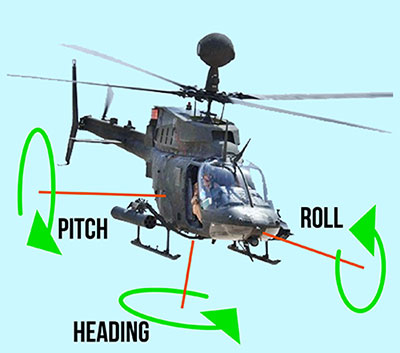
\includegraphics[width=0.30\textwidth]{figures/pitch-roll-heading.jpg}
    \caption{Orientação espacial de uma aeronave: arfagem (\textit{pitch}), rolagem (\textit{roll}) e guinada (\textit{heading}).}
    \label{fig:helicoptero}
\end{figure}
